The application is a self-contained web service: \texttt{python app/server.py} (or \texttt{run\_app.bat}) starts a FastAPI server on \texttt{127.0.0.1:8000}, loads the target and draft models and merges the LoRA adapters in a background thread, and serves a single-page browser interface; no notebook, command-line step or IDE is needed afterwards. The header shows a status indicator (starting, ready, error), the loaded model and adapter, and a persistent banner states that this is an educational screening prototype and not a clinical enrollment decision. Loading takes well under a minute on the laptop; requests that arrive earlier receive a clear ``model not ready'' message instead of an error. If an adapter is missing, the base model is used and the header says so.

\textbf{Screening workflow (Fig.~\ref{fig:app2}).} A user supplies a patient note by pasting text or loading one of the held-out sample patients, and a trial by choosing a sample trial, fetching one from ClinicalTrials.gov by NCT identifier (public metadata only), pasting an ``Inclusion Criteria / Exclusion Criteria'' block that is split into individual criteria, or typing criteria manually. Notes that are not already numbered are split into sentences and numbered from zero, with a preview of the numbering. For every criterion the interface shows the predicted label, the cited sentences quoted from the note, an explanation that only restates the label and the cited text, the raw model output, latency and generated tokens, and, for the sample patients, the dataset's expert label with a match indicator; selecting a criterion highlights its cited sentences in the numbered note (yellow) and the expert's sentences (green marker). The preliminary outcome (here ``Needs more information'') is computed by the explicit rule of Section~III-H and is displayed together with that rule. Missing information is never presented as eligibility: a criterion with no cited sentence is shown with the text ``No supporting sentence cited''.

\textbf{Report export and provenance.} The \emph{Download report} buttons produce a readable HTML report (also suitable for printing to PDF), a Markdown file or a JSON file containing the disclaimer, the trial, the preliminary outcome with its rule, every criterion with label, evidence text and explanation, the numbered note, and provenance: generation time, model, a SHA-256 prefix of the adapter file, the decoding settings and a hash of the note.

\textbf{Input validation and recovery (Fig.~\ref{fig:app3}).} The server validates every request: notes shorter than 20 characters, unknown criterion types, criteria shorter than 3 characters or empty reports are rejected with an explanatory message and HTTP~422; an unreachable registry yields a message asking the user to paste the criteria instead; prompts above 3\,000 tokens are refused rather than silently truncated; and if one criterion fails during a multi-criterion run it is reported as invalid while the others continue. After an error the user corrects the field and runs again without reloading.

\textbf{Inference comparison (Fig.~\ref{fig:app4}).} The \emph{Compare decoding} tab runs the current note and a chosen criterion through the four implemented modes---uncached reference, KV cache, KV cache with tiled attention, and speculative decoding with a selectable draft length---with a warm-up pass and selectable repetitions, optionally forcing a longer output. It reports whether each mode's tokens are identical to the first, prefill, decode and total time, tokens per second, speed-up, memory growth, target forward passes and, for speculative decoding, the acceptance rate, and draws latency and throughput bars. These numbers are measured live on the machine hosting the application, not read from images; the \emph{Experiments} tab additionally renders the stored result files (before/after metrics, KV, attention and speculative benchmarks). In the screenshot, taken while a training job was competing for the same CPU, all four modes return identical tokens, the cache is faster than the reference, our tiled kernel is slower than SDPA inside the decoder, and speculative decoding reaches a 41\% acceptance rate with the un-tuned draft available at that moment.

\begin{figure}[t]\centering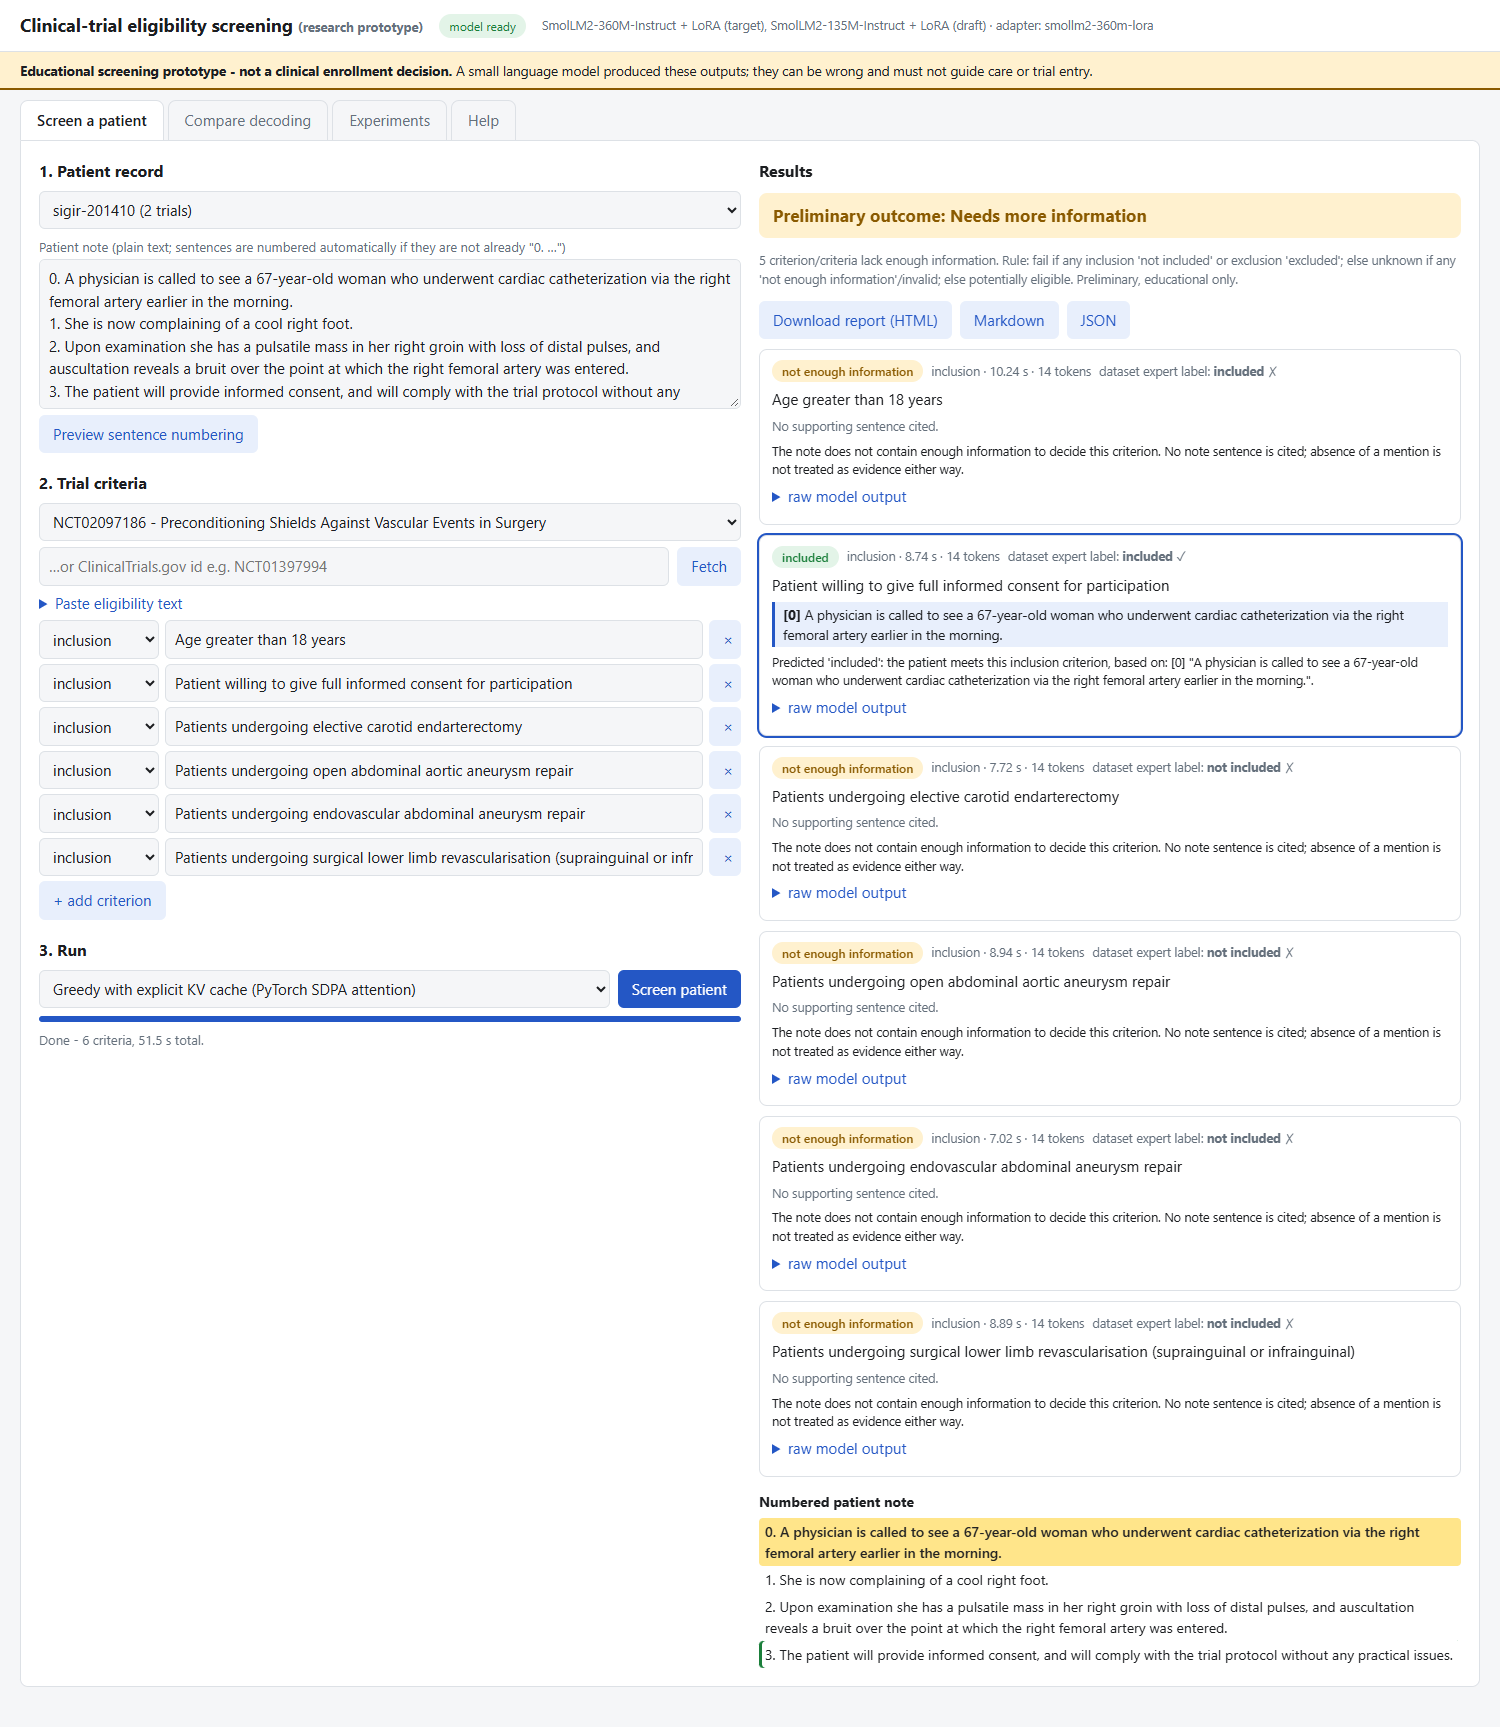
\includegraphics[height=.52\textheight,keepaspectratio]{app_02_results.png}
\caption{Screening workflow: sample patient and trial, six criteria screened, per-criterion label and cited evidence, preliminary outcome, report export buttons, and the numbered note with the selected criterion's evidence highlighted.}\label{fig:app2}\end{figure}
\begin{figure}[t]\centering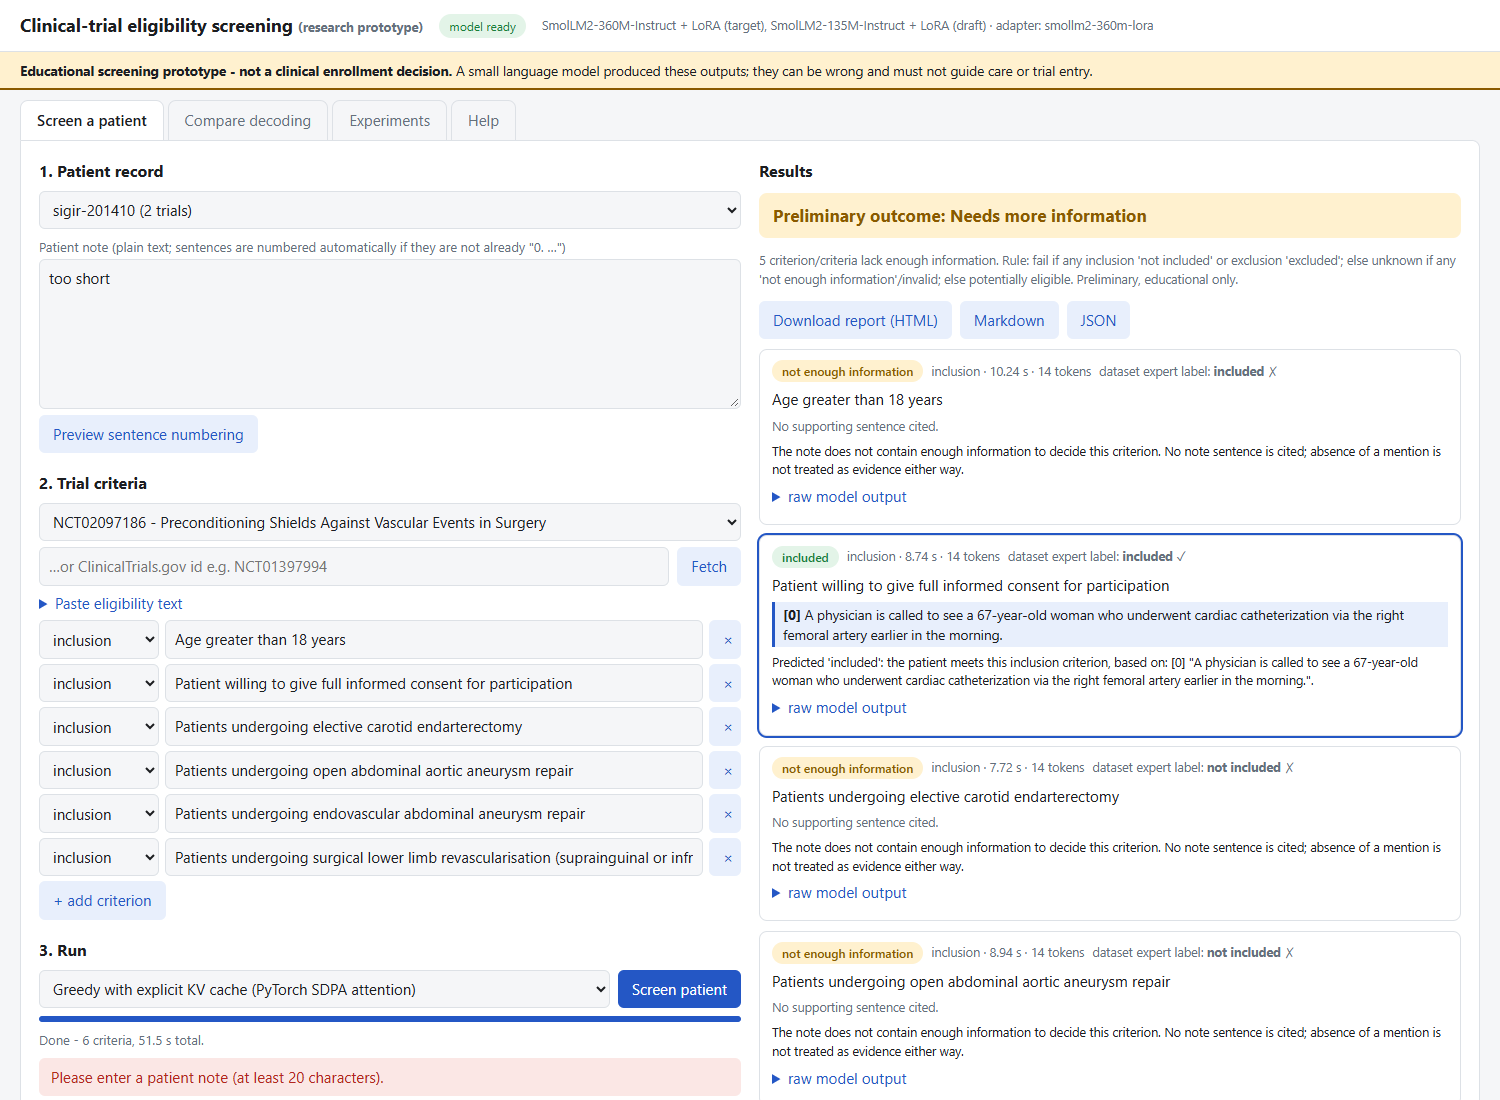
\includegraphics[width=\columnwidth]{app_03_error_recovery.png}
\caption{Recovery from an invalid input: a too-short note is rejected with an explanatory message and the form remains usable.}\label{fig:app3}\end{figure}
\begin{figure}[t]\centering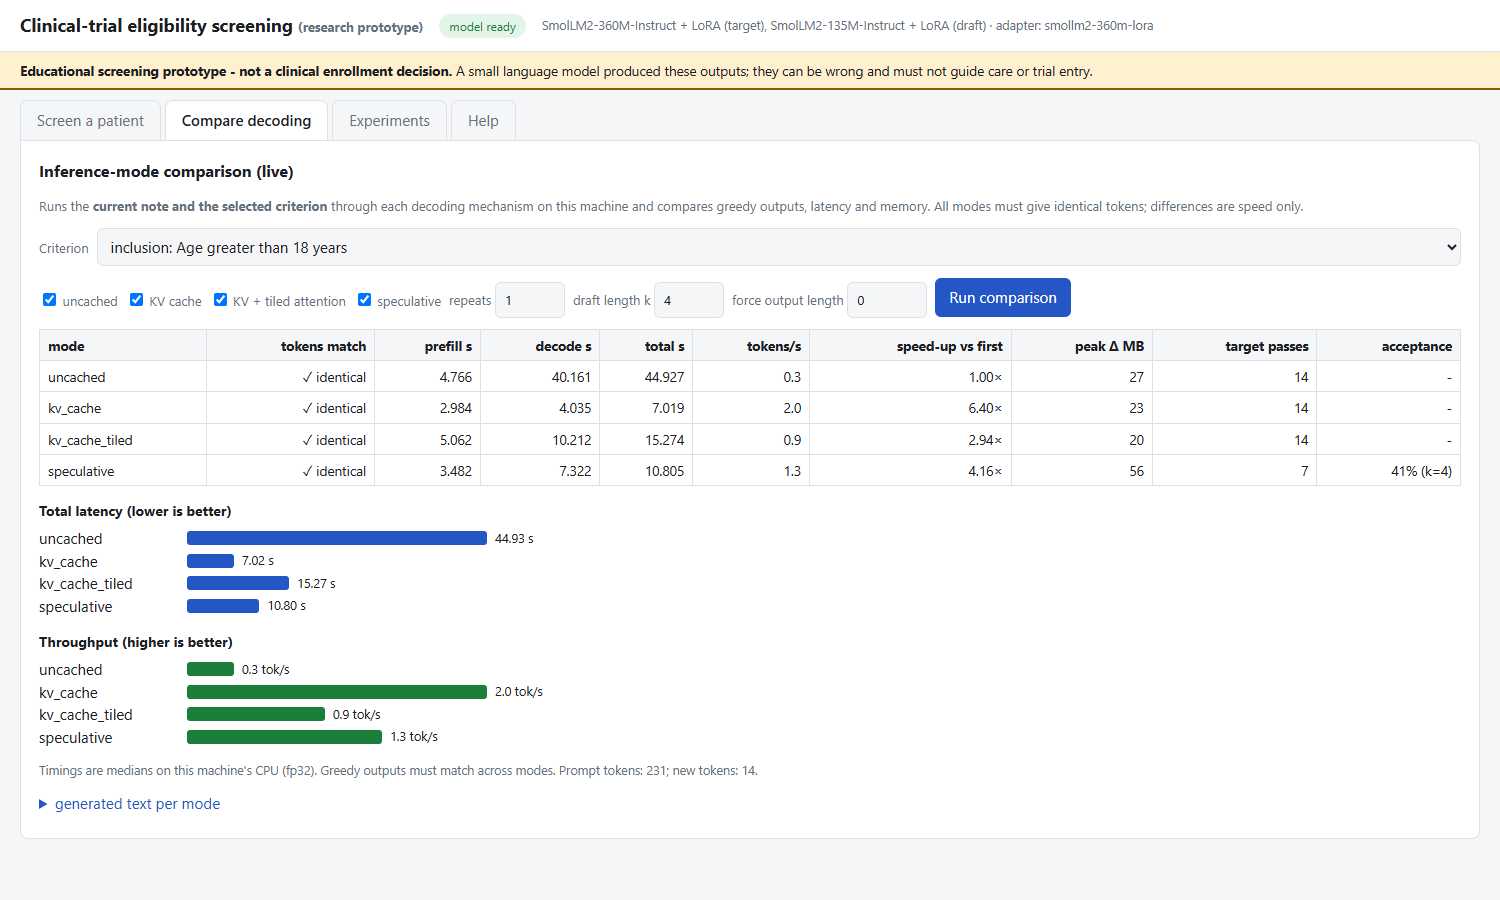
\includegraphics[width=\columnwidth]{app_04_compare.png}
\caption{\emph{Compare decoding} tab: live comparison of the four decoding modes on the same input (timings include contention from a concurrent training job).}\label{fig:app4}\end{figure}
